\chapter{Resultados}
\epigraph{\textit{Do or do not, there is no try.}}{-Master Yoda}
\label{section:Resultados}
Este capítulo apresenta os resultados das etapas do fluxo proposto, bem como a análise dos mesmos. Alguns resultados preliminares foram utilizados para verificar se o trabalho estava coerente com a base teórica anteriormente exposta. Outros auxiliaram na análise do fluxo de envelhecimento e na acuidade dos métodos de estimativa propostos.

Algumas considerações precisam ser feitas antes da análise dos dados. O ambiente de simulação criado para este trabalho utiliza ferramentas de EAD previamente disponíveis para degradação, sendo sua integração realizada através de um conjunto de \textit{scripts} ou \textit{wrappers}, que são responsáveis por automatizar:
\begin{enumerate}
	\item A criação das diversas netlists utilizadas no fluxo;
	\item Formatação dos arquivos utilizados como banco de dados bem como preenchimento dos mesmos;
	\item A passagem de parâmetros de entrada às ferramentas de EAD;
	\item A extração dos resultados de simulação;
	\item A atualização do banco de dados com os resultados de estimativas de MTTF.
\end{enumerate}

\section{Caracterização de células}
\label{section:caracterização}
Para investigar a relação entre as condições ambientais e a degradação de sistemas, é preciso averiguar primeiramente se é possível reproduzir resultados que estejam coerentes com a literatura. Isso significa que é necessário garantir que, ao se degradar um sistema, as alterações nas condições ambientais (\textit{p.ex.} temperatura) sejam refletidas no sistema conforme esperado. É bem estabelecido que uma alteração na tensão de alimentação $V_{DD}$ e na temperatura deve influenciar não só a operação dos dispositivos mas também na contribuição dos efeitos de degradação expostos na seção \ref{subsection_Conf_CI}. Esta premissa precisa então ser satisfeita.

Com este propósito foram caracterizadas as seguintes células básicas: INV (inversor), AND2, OR2, NOR2 e NAND2. Todas as células foram submetidas a BDPEs estáticos e populados exclusivamente para estas simulações. Por estático indica-se que a célula foi submetida a uma mesma temperatura e tensão ao longo de toda a simulação ao invés de diferentes $T_{conj,X}$ e $V_{conj,Y}$. Cada BDPE possui 200 perfis e o tempo de degradação para todas as células é de 1 ano.

Foram criados 5 BDPE's diferentes, um para cada célula. Entretanto, todos os perfis foram gerados usando a mesma premissa: os valores de temperatura seguem uma distribuição normal de média $\mu = 80$ e desvio-padrão $\sigma=10$. Os valores de tensão também seguem uma distribuição normal, porém de média $\mu = 1.1$ e desvio-padrão $\sigma=0.2$. Foi escolhida uma média de 80$^{\circ}$C com o intuito de garantir uma contribuição significativa da temperatura na degradação. Já a média da tensão de alimentação de $1.1V$ está de acordo com os parâmetros da tecnologia dos transistores utilizados na simulação.

Após cada célula ter sido degradada, o atraso de saída $\Delta t_d$ para cada perfil simulado foi adicionado aos seus respectivos BDPEs e foi criado um modelo de regressão linear múltipla para cada. Os modelos foram utilizados para plotar a dependência do atraso de saída pela tensão de operação e pela temperatura. Os resultados estão representados nas figuras \ref{figure:delays_inv_caracterizacao_200Pontos_gauss80_10} a \ref{figure:delays_or2_caracterizacao_200Pontos_gauss80_10}.
\begin{figure}[H]
\center
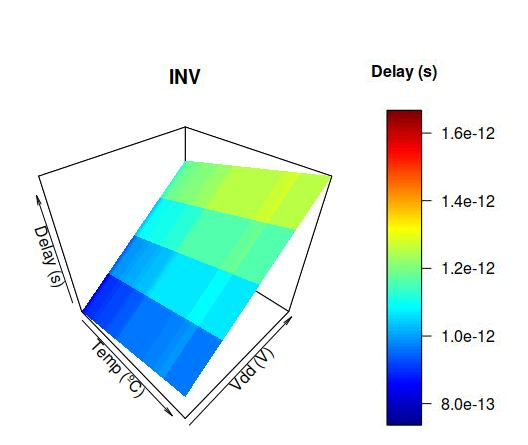
\includegraphics[width=0.6\textwidth]{images/delays_inv_caracterizacao_200Pontos_gauss80_10}
\caption{Caracterização de uma célula inversora degradada durante 1 ano.}
\label{figure:delays_inv_caracterizacao_200Pontos_gauss80_10}	
\end{figure}
A figura \ref{figure:delays_inv_caracterizacao_200Pontos_gauss80_10} mostra que, à medida que a temperatura sobre o inversor (dada em $^{\circ}$C) aumenta, o atraso $\Delta t_d$ (dado em segundos) também incrementa. Entretanto, a influência da temperatura é menor se comparada à da tensão de alimentação, o que era esperado.

Para esta análise, os coeficientes da regressão linear múltipla (e consequentemente a influência de cada grandeza) são dados pelos valores da tabela \ref{tb:regressao_multipla_INV}:
\begin{table}[H]
	\centering
	\caption{Coeficientes do modelo de RLM para o inversor da figura \ref{figure:delays_inv_caracterizacao_200Pontos_gauss80_10}.}
	\begin{tabular}{@{}l|l|l|l@{}}
		\toprule
		& Interceptação & $T_{conj,1}$ & $V_{conj,1}$ \\ \midrule
		Coeficiente & $-1.3049e^{-12}$ & $5.0378e^{-15}$ & $1.9161e^{-12}$ \\ \bottomrule
	\end{tabular}
	\label{tb:regressao_multipla_INV}
\end{table}
Do modelo fica claro que a influência da tensão sobre o envelhecimento é 3 ordens de grandeza maior que a da temperatura. Uma relação semelhante foi encontrada para as células AND2, NAND2, OR2 e NOR2.
\begin{figure}[H]
	\center
	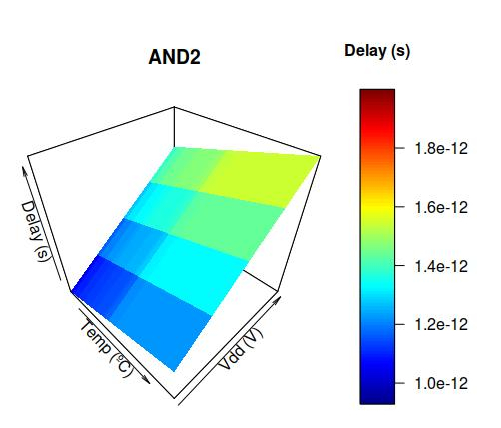
\includegraphics[width=0.6\textwidth]{images/delays_and2_caracterizacao_200Pontos_gauss80_10}
	\caption{Caracterização de uma célula AND2 degradada durante 1 ano.}
	\label{figure:delays_and2_caracterizacao_200Pontos_gauss80_10}	
\end{figure}
\begin{table}[H]
	\centering
	\caption{Coeficientes do modelo de RLM para a figura \ref{figure:delays_and2_caracterizacao_200Pontos_gauss80_10}.}
	\begin{tabular}{@{}l|l|l|l@{}}
		\toprule
		& Interceptação & $T_{conj,1}$ & $V_{conj,1}$ \\ \midrule
		Coeficiente & $-1.4112e^{-12}$ & $5.8058e^{-15}$ & $2.1905e^{-12}$ \\ \bottomrule
	\end{tabular}	
	\label{tb:regressao_multipla_AND2}
\end{table}
\begin{figure}[H]
	\center
	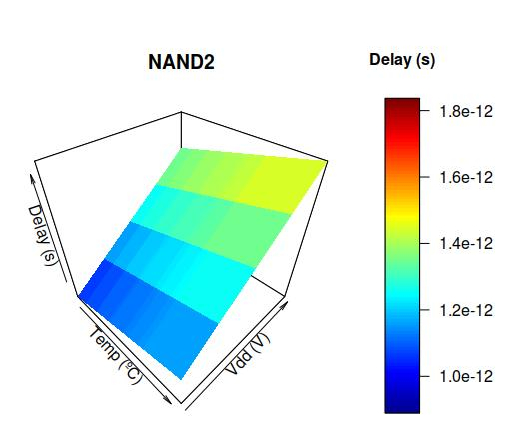
\includegraphics[width=0.6\textwidth]{images/delays_nand2_caracterizacao_200Pontos_gauss80_10}
	\caption{Caracterização de uma célula NAND2 degradada durante 1 ano.}
	\label{figure:delays_nand2_caracterizacao_200Pontos_gauss80_10}	
\end{figure}
\begin{table}[H]
	\centering
	\caption{Coeficientes do modelo de RLM para a figura \ref{figure:delays_nand2_caracterizacao_200Pontos_gauss80_10}.}
	\begin{tabular}{@{}l|l|l|l@{}}
		\toprule
		& Interceptação & $T_{conj,1}$ & $V_{conj,1}$ \\ \midrule
		Coeficiente & $-1.2030e^{-12}$ & $5.5807e^{-15}$ & $1.9283e^{-12}$ \\ \bottomrule
	\end{tabular}
	\label{tb:regressao_multipla_NAND2}
\end{table}
\begin{figure}[H]
	\center
	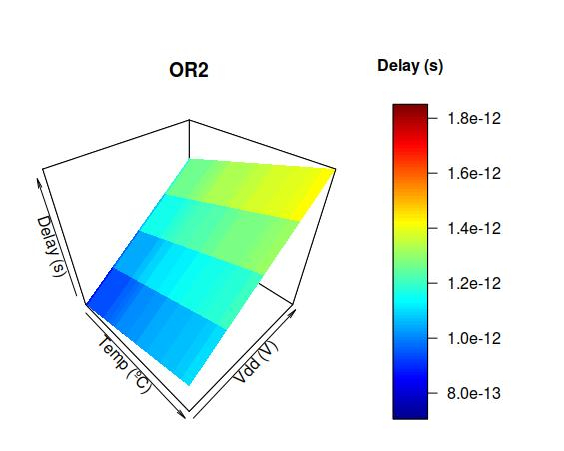
\includegraphics[width=0.6\textwidth]{images/delays_or2_caracterizacao_200Pontos_gauss80_10}
	\caption{Caracterização de uma célula OR2 degradada durante 1 ano.}
	\label{figure:delays_or2_caracterizacao_200Pontos_gauss80_10}	
\end{figure}
\begin{table}[H]
	\centering
	\caption{Coeficientes do modelo de RLM para a figura \ref{figure:delays_or2_caracterizacao_200Pontos_gauss80_10}.}
	\begin{tabular}{@{}l|l|l|l@{}}
		\toprule
		& Interceptação & $T_{conj,1}$ & $V_{conj,1}$ \\ \midrule
		Coeficiente & $-1.5102e^{-12}$ & $5.9055e^{-15}$ & $2.1376e^{-12}$ \\ \bottomrule
	\end{tabular}
	\label{tb:regressao_multipla_OR2}
\end{table}
\begin{figure}[H]
	\center
	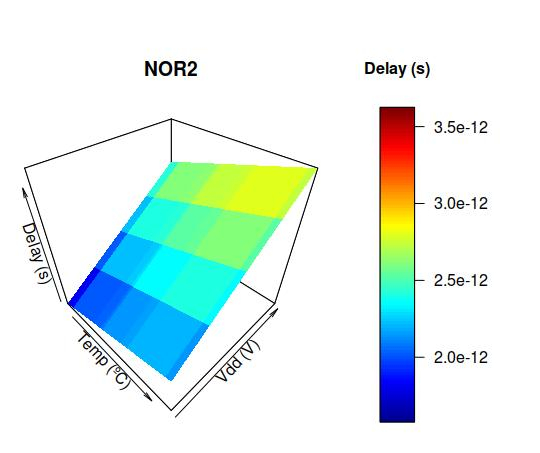
\includegraphics[width=0.6\textwidth]{images/delays_nor2_caracterizacao_200Pontos_gauss80_10}
	\caption{Caracterização de uma célula NOR2 degradada durante 1 ano.}
	\label{figure:delays_nor2_caracterizacao_200Pontos_gauss80_10}	
\end{figure}
\begin{table}[H]
	\centering
	\caption{Coeficientes do modelo de RLM para a figura \ref{figure:delays_or2_caracterizacao_200Pontos_gauss80_10}.}
	\begin{tabular}{@{}l|l|l|l@{}}
		\toprule
		& Interceptação & $T_{conj,1}$ & $V_{conj,1}$ \\ \midrule
		Coeficiente & $-2.9256e^{-12}$ & $1.3332e^{-14}$ & $4.0494^{-12}$ \\ \bottomrule
	\end{tabular}
	\label{tb:regressao_multipla_OR2}
\end{table}

Era esperado que a relação entre tensão de alimentação e atraso fosse positiva. O mesmo pode ser dito entre a temperatura e o atraso. Estes resultados iniciais nos dão segurança de que o fluxo está pronto e que ele pode ser utilizado para sistemas maiores. Além disso, eles confirmam aquilo que já era esperado: quando da utilização do método de correlação, descrito na seção \ref{subsection_estimativas_correlacao}, devemos procurar pelo resultado de maior correlação positiva, já que o atraso cresce com o aumento da temperatura e tensão.
\section{Degradação de circuitos de teste}
\label{section:caracterização_iscas}
Uma vez realizados testes com células básicas, mais circuitos foram utilizados para continuar investigando a viabilidade do fluxo e da metodologia. Com esse intuito, foram utilizados quatro circuitos ISCAS-85: c499, c880, c1355, c5315. Esses circuitos ISCAS são implementações de blocos combinacionais pré-determinados cujo objetivo é propor circuitos padrões para testes de diferentes propósitos \cite{Hansen1999}. A função implementada e a respectiva quantidade de portas lógicas para cada um deles está descrita na tabela \ref{tb:ISCAS_85}.

\begin{table}[H]
\centering
\caption{Características da cadeia de inversores e dos circuitos ISCAS-85 utilizados \cite{Hansen1999}.}
\begin{tabular}{@{}lll@{}}
\toprule
Circuito & Função & Qtde. de portas \\ \midrule
inv100 & Cadeia de Inversores & \ \ \ \ 100 \\ \midrule
c499 & Single-Error-Correcting de 32-bit & \ \ \ \ 474 \\ \midrule
c880 & ULA de 8 bits & \ \ \ \ 393 \\ \midrule
c1355 & Single-Error-Correcting de 32-bit & \ \ \ \ 738 \\ \midrule
c5315 & ULA de 9 bits & \ \ \ \ 1781 \\ \bottomrule
\end{tabular}
\label{tb:ISCAS_85}
\end{table}
Esses circuitos podem ser utilizados para os próximos passos em sua integridade ou apenas uma porção dos mesmos. Por integridade entende-se que os circuitos, inicialmente descritos através de uma linguagem de descrição de hardware (Hardware Description Language, HDL), serão sintetizados e uma netlist esquemática no formato Spectre criada. 

Por porção entende-se que somente uma parte do circuito será utilizada para criação da netlist Spectre. Esta parte deve ser capaz de, após as simulações de degradação, representar o pior caso para o restante do circuito. Esta porção pode ser representada por um ou mais caminhos críticos, conforme exposto na seção \ref{section_extracao_caminhos}.
Foram extraídos os caminhos críticos dos circuitos ISCAS da tabela \ref{tb:ISCAS_85} e netlists esquemáticas menores foram criadas a partir destes caminhos.

Para extração dessa informação, foi utilizada uma funcionalidade nativa da ferramenta de síntese capaz de relatar quais são os caminhos críticos de um circuito. Além disso, eles devem ser ativados de tal forma que uma transição na saída seja detectável. Isso significa que as portas lógicas serão ativadas ou desativadas em uma combinação específica que reflita não só o maior atraso de propagação possível mas também uma mudança lógica na saída do caminho crítico.

Após a extração destes caminhos, os circuitos foram reduzidos aos tamanhos descritos na tabela \ref{tb:tamanho_piores_caminhos}.
\begin{table}[H]
	\centering
	\caption{Tamanho dos circuitos de teste após a extração dos caminhos críticos.}
	\begin{tabular}{@{}ll@{}}
		\toprule
		Circuito & Qtde. de portas \\ \midrule
		inv100 & \ \ \ \ 100 \\ \midrule
		w\_c499 & \ \ \ \ 10 \\ \midrule
		w\_c880 & \ \ \ \ 8 \\ \midrule
		w\_c1355 & \ \ \ \ 21 \\ \midrule
		w\_c5315 & \ \ \ \ 25 \\ \bottomrule
	\end{tabular}
	\label{tb:tamanho_piores_caminhos}
\end{table}
O sufixo ``w\_'' foi adicionado aos nomes dos ISCAS unicamente como forma de diferenciar os circuitos com caminhos críticos (\textit{p. ex.} w\_c499) dos seus respectivos circuitos completos. Após a extração dos caminhos, um circuito de teste (\textit{testbench}) foi criado para cada um dos circuitos da tabela \ref{tb:tamanho_piores_caminhos} cujo objetivo é ativar o caminho crítico, conforme mencionado anteriormente.  

Uma vez criadas, as netlists são padronizadas com valores de temperatura $T=0$ e alimentação $V_{DD}=0.0$. Eles são utilizados como referência pelos \textit{scripts}, substituindo estes valores pelos respectivos $T_{conj,X}$ e $V_{conj,Y}$ durante a simulação.

Como exemplo, considere que a tabela \ref{tb:regressao_multipla_exemplo2} possui perfis de envelhecimento para o circuito $w\_c499$. Para o primeiro perfil, serão criadas $N=14$ netlists, das quais 13 serão submetidas a uma temperatura $T=30^{\circ}C$ e uma a $T=50^{\circ}C$. Já para $V_{DD}$, 12 estarão submetidas a uma tensão $V_{DD}=1.0V$ e duas a $V_{DD}=1.1V$. Dessa forma, as 12 primeiras netlists terão os valores $T=0$ e $V_{DD}=0.0$ substituídos por $T=30^{\circ}C$ e alimentação $V_{DD}=1.0V$. A 13º netlist terá $T=30^{\circ}C$ e $V_{DD}=1.1V$. A restante terá $T=50^{\circ}C$ e $V_{DD}=1.1V$.

Cada circuito foi submetido a um BDPE de aproximadamente 250 entradas cujos perfis são submetidos aos conjuntos de condições ambientais $T_{conj,X}=[10, 30, 50, 70, 90]$ e $V_{conj,Y}=[0.9, 1.0, 1.1, 1.2, 1.3]$. Os valores de $p_{T(w,x)}$ e $p_{V(w,y)}$ foram gerados pseudo-aleatoriamente, sendo $\sum p_{T(w,x)}=100$ e $\sum p_{V(w,y)}=100$ (ou seja, $N=100$). Assim sendo, cada entrada do BDPE corresponde a 100 degradações, totalizando 2500 simulações de envelhecimento para toda o banco de dados de perfis e que são posteriormente adicionados ao BDPE, conforme descrito no capítulo 4.

Uma segunda bateria de testes é realizada, porém com condições ambientais diferentes. Os mesmos circuitos são degradados mas desta vez submetidos a um BDPE estático. Isso significa que o perfil ao qual são submetidos permanece 100\% do tempo em um único $T_{conj,X}$ e um único $V_{conj,Y}$. Esse comportamento é representado através da criação de uma tabela de perfis, representada na tabela \ref{tb:BDPE_estatico}.

\begin{table}[H]
	\centering
	\caption{BDPE estático utilizado no envelhecimento dos circuitos de teste.}
	\begin{tabular}{@{}l|l|l|l|l|l@{}}
		\toprule
		$40$ & $70$ & $100$ & $1.0$ & $1.1$ & $1.2$ \\ \midrule
		$3$ & $0$ & $0$ & $3$ & $0$ & $0$ \\
		$0$ & $3$ & $0$ & $3$ & $0$ & $0$ \\
		$0$ & $0$ & $3$ & $3$ & $0$ & $0$ \\
		$3$ & $0$ & $0$ & $0$ & $3$ & $0$ \\
		$0$ & $3$ & $0$ & $0$ & $3$ & $0$ \\
		$0$ & $0$ & $3$ & $0$ & $3$ & $0$ \\
		$3$ & $0$ & $0$ & $0$ & $0$ & $3$ \\
		$0$ & $3$ & $0$ & $0$ & $0$ & $3$ \\
		$0$ & $0$ & $3$ & $0$ & $0$ & $3$ \\
		\bottomrule
	\end{tabular}
	\label{tb:BDPE_estatico}
\end{table}
Este tipo de teste auxilia a investigar melhor quais são as vantagens da metodologia proposta ao comparar os resultados anteriores com os de uma abordagem de perfis estáticos. É preciso esclarecer primeiramente que um perfil definido por $T_{conj,X}=[40,70,100]$ e $p_{T(1,x)}=[3,0,0]$, utilizando a tabela \ref{tb:BDPE_estatico} como exemplo, não necessariamente indica que um sistema foi degradado sob influência de uma temperatura e tensão constantes. Para um sistema real não é possível assumir essa premissa. Entretanto, o perfil de temperatura e tensão podem, por escolha do projetista, ser representados por médias (\textit{p.ex} temperatura média ou tensão de alimentação média).

Dessa forma, é possível avaliar se a representação estática da operação do sistema oferece uma precisão semelhante à representação dinâmica. Se for possível representar o perfil de um sistema através de uma estatística simples (como as médias) e obter um erro de predição semelhante ou melhor do que a dinâmica, então deve-se questionar a utilização de um BDPE dinâmico, já que não existiria, em tese, uma redução do erro. Esta análise também será realizada nas seções subsequentes.
\section{Métricas e estatísticas}
\label{section:metricas_estatisticas}
Antes de explorar os dados de simulação, é preciso explicar quais métricas foram utilizadas para este trabalho. Uma métrica, no contexto aqui apresentado, deve ser capaz de indicar a precisão ou assertividade dos métodos de estimativa apresentados na seção \ref{section_metodos_estimativa}, dando uma perspectiva diferenciada dos resultados. Qual métrica se mostra mais adequada é um debate que não faz parte deste trabalho, visto que não há consenso na literatura específica da área \cite{Poli1993}\cite{Willmott}\cite{Chai2014}. Ao invés disso, mais de uma métrica será utilizada, cabendo ao projetista julgar a mais adequada ao entendimento de seus dados.

A análise gráfica dos resultados utilizará apenas algumas destas métricas. Entretanto serão sumarizadas, ao longo da análise, as seguintes métricas: Erro Relativo (ER), Erro Máximo (EMAX), Erro Quadrático Médio (EQM) e Erro Normalizado da Raiz do Valor Quadrático Médio (ENRVQM). Estas métricas são expressas por:
\begin{align}
ER = 100\left(1 - \frac{\hat{y_i}}{y_i}\right) \\
EMAX = \max{\left(100\left(1 - \frac{\hat{y_i}}{y_i}\right)\right)} \\
EQM = \frac{\sum_{i=1}^{n}(\hat{y_i}-y_i)^2}{n} \\
ENRVQM = \frac{\sqrt{EQM}}{\bar{y}}
\end{align}
onde $n$ representa a quantidade de observações, $\bar{y}$ é a média dos dados observados, $\hat{y_i}$ é o i-ésimo dado observado e $y_i$ o i-ésimo dado estimado.
Por ser a mais simples e intuitiva, o ER é a primeira métrica a ser explorada adiante.

Apesar de dispormos destas essas métricas, é interesse evitar que um modelo de estimativa não sofra com um efeito de sobreajuste, ou seja, ele tente se acomodar demasiadamente aos dados observados, reduzindo a performance do modelo e consequentemente afetando as métricas mencionadas acima.

Para evitar o sobreajuste, foi utilizado uma técnica de validação cruzada. Esta abordagem propõe dividir os dados pré-existentes em dois grupos: dados de treino e dados de teste. Os dados de treinamento são utilizados para obtenção do modelo preditivo. Já os dados de teste são utilizados para medir a precisão do modelo. A técnica de validação cruzada escolhida para a análise foi \textit{leave-one-out cross-validation} (LOOCV), onde apenas uma das amostras é utilizada como teste e as restantes são utilizadas como dados de treino \cite{James2013}.

Utilizemos a tabela \ref{tb:exemplo_cross_validation}, que é um excerto de um dos BDPE utilizados neste trabalho, como exemplo.  
\begin{table}[H]
	\centering
	\caption{Excerto de um BDPE com dados de simulação.}
	\begin{tabular}{@{}l|l|l|l|l|l|l|l|l|l|l@{}}
		\toprule
		$10$ & $30$ & $50$ & $70$ & $90$ & $0.9$ & $1.0$ & $1.1$ & $1.2$ & $1.3$ & MTTF \\ \midrule
		$37$ & $56$ & $1$ & $6$ & $0$ & $37$ & $56$ & $1$ & $6$ & $0$ & $1.46$ \\
		$70$ & $0$ & $7$ & $0$ & $23$ & $70$ & $0$ & $7$ & $0$ & $23$ & $1.13$ \\
		$47$ & $0$ & $0$ & $42$ & $11$ & $47$ & $0$ & $0$ & $42$ & $11$ & $1.15$ \\
		\bottomrule
	\end{tabular}
	\label{tb:exemplo_cross_validation}
\end{table}
Na técnica de LOOCV a primeira amostra (linha 2 da tabela \ref{tb:exemplo_cross_validation}) é retirada, por exemplo, restando somente 2 entradas para criação do modelo preditivo, seja ele PLS-R, DE ou COR. Após criado, a amostra retirada é usada como entrada no modelo e o resultado estimado $\hat{y_1}$ é comparado ao esperado $y_1$. Nesse exemplo, considerando um tempo de operação $t_{oper}=1$ ano, é conhecido que, para um perfil $p_{T(1,x)}=[37,56,1,6,0]$ e $p_{V(1,y)}=[37,56,1,6,0]$, o resultado esperado é $y_1=1.46$ (MTTF de 1.46 anos). A partir daí, as métricas de erro anteriormente mencionadas podem se utilizadas para medir a precisão dos métodos.

Para se obter métricas mais significativas ainda, a LOOCV foi utilizada $N$ vezes, onde $N$ é quantidade de amostras do BDPE. Isso significa que, após a primeira amostra ser utilizada como teste e os erros serem calculados, a LOOCV é repetida mas desta vez usando a segunda amostra como teste e assim sucessivamente. Todos os resultados são utilizados para compor as métricas mencionadas. Dessa forma não se está testando um modelo específico obtido através de um método de distância euclideana, por exemplo, mas está sendo testado ``exaustivamente'' a DE como método de estimativa.

É importante salientar que durante a operação real do sistema, ao contrário do ambiente de simulação, o modelo já será conhecido no momento em que a predição for necessária, pois já foi previamente treinado. O perfil que é utilizado na análise \textit{online} como entrada para o modelo é proveniente do BDM (e não do BDPE).
\section{Resultados das simulações dos circuitos de teste}
A primeira métrica analisada foi o erro relativo, como forma de compreender a exatidão dos métodos. Levando em consideração que o ``verdadeiro'' valor do MTTF é conhecido, o erro relativo em valores absolutos para o BDPE descrito na seção \ref{section:caracterização_iscas} é representado pelos diagramas de caixa das figuras \ref{figure:ER_MTTF} e \ref{figure:erro_relativo_MTTF_inv100_random}.
\begin{figure}[H]
	\subfloat[ER para pior caminho do ISCAS c499\label{figure:erro_relativo_MTTF_worst_c499_random2}]{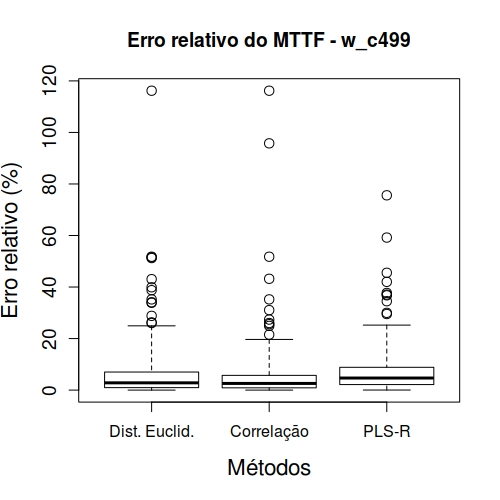
\includegraphics[width=0.5\textwidth]{images/erro_relativo_MTTF_worst_c499_random2}
	}
	\hfill
	\subfloat[ER para pior caminho do ISCAS c880\label{figure:erro_relativo_MTTF_worst_c880_random2}]{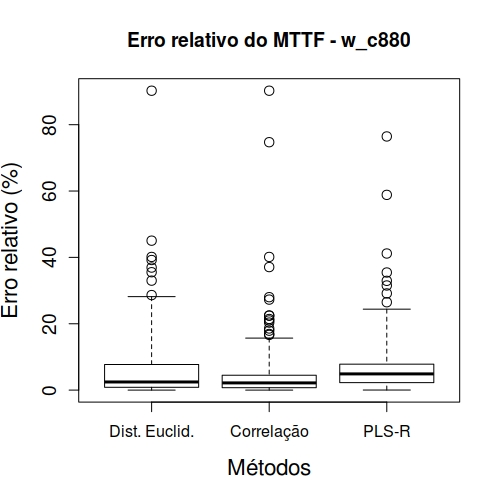
\includegraphics[width=0.5\textwidth]{images/erro_relativo_MTTF_worst_c880_random2}
	}
	\hfill
	\subfloat[ER para pior caminho do ISCAS c1355\label{figure:erro_relativo_MTTF_worst_c1355_random2}]{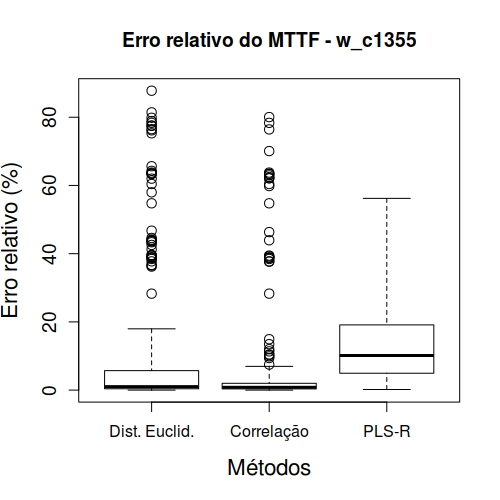
\includegraphics[width=0.5\textwidth]{images/erro_relativo_MTTF_worst_c1355_random2}
	}
	\hfill
	\subfloat[ER para pior caminho do ISCAS c5315\label{figure:erro_relativo_MTTF_worst_c5315_random2}]{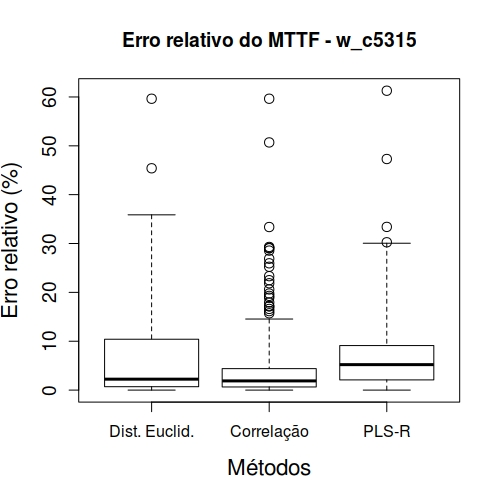
\includegraphics[width=0.5\textwidth]{images/erro_relativo_MTTF_worst_c5315_random2}
	}
	\caption{Erro relativo do MTTF para os circuitos ISCAS-85.}
	\label{figure:ER_MTTF}
\end{figure}
\begin{figure}[H]
	\center
	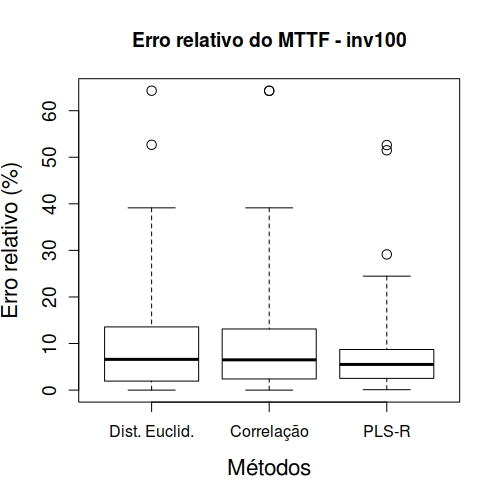
\includegraphics[width=0.5\textwidth]{images/erro_relativo_MTTF_inv100_random}
	\caption{Erro relativo do MTTF para a cadeia de inversores.}
	\label{figure:erro_relativo_MTTF_inv100_random}	
\end{figure}

Extraindo o EMAX (como uma porcentagem) para cada circuito e método obtém-se:

\begin{table}[H]
	\centering
	\caption{Erro máximo para os circuitos de teste.}
	\begin{tabular}{@{}l|l|l|l@{}}
		\toprule
		Circuito & Dist. Eucli. & Cor. & PLS-R \\ \midrule
		inv100 & \ \ \ 64.29\% & 64.29\% & 52.61\% \\
		w\_c499 & \ \ \ 116.21\% & 116.21\% & 75.61\% \\
		w\_c880 &  \ \ \ 90.24\% & 90.24\% & 76.45\% \\
		w\_c1355 & \ \ \ 80.05\% & 87.78\% & 56.21\% \\
		w\_c5315 & \ \ \ 59.64\% & 59.64\% & 61.28\% \\
		\bottomrule
	\end{tabular}
	\label{tb:erro_maximo_ISCAS}
\end{table}

Para obter uma comparação mais intuitiva, o Erro Quadrático Médio (EQM) foi calculado para cada um dos circuitos e por fim normalizado, servindo como um rápido indicativo de qual método é mais preciso e o quão mais preciso é em comparação aos demais. 
\begin{figure}[H]
	\subfloat[EQMN para pior caminho do ISCAS c499\label{figure:NMSE_MTTF_worst_c499_random2}]{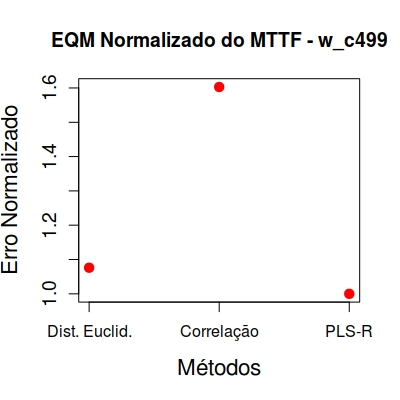
\includegraphics[width=0.5\textwidth]{images/NMSE_MTTF_worst_c499_random2}
	}
	\hfill
	\subfloat[EQMN para pior caminho do ISCAS c880\label{figure:NMSE_MTTF_worst_c880_random2}]{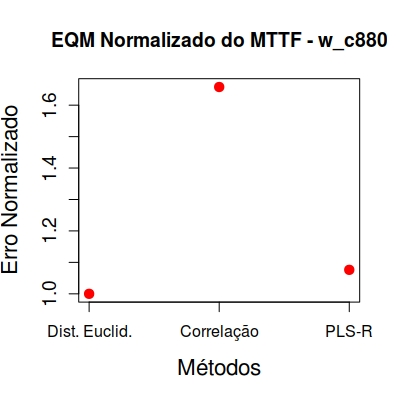
\includegraphics[width=0.5\textwidth]{images/NMSE_MTTF_worst_c880_random2}
	}
	\hfill
	\subfloat[EQMN para pior caminho do ISCAS c1355\label{figure:NMSE_MTTF_worst_c1355_random2}]{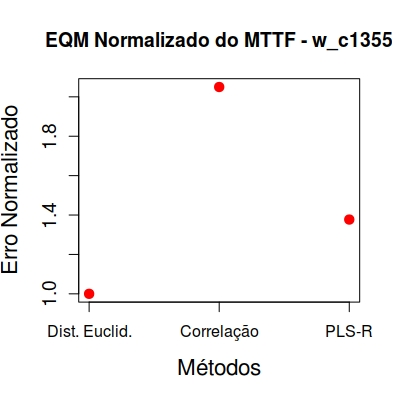
\includegraphics[width=0.5\textwidth]{images/NMSE_MTTF_worst_c1355_random2}
	}
	\hfill
	\subfloat[EQMN para pior caminho do ISCAS c5315\label{figure:NMSE_MTTF_worst_c5315_random2}]{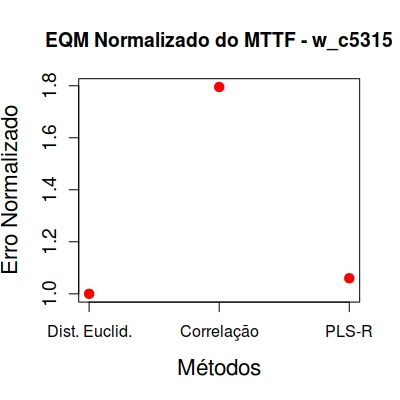
\includegraphics[width=0.5\textwidth]{images/NMSE_MTTF_worst_c5315_random2}
	}
	\caption{Erro Quadrático Médio Normalizado do MTTF para os circuitos ISCAS-85.}
	\label{figure:NMSE_MTTF}
\end{figure}
\begin{figure}[H]
	\center
	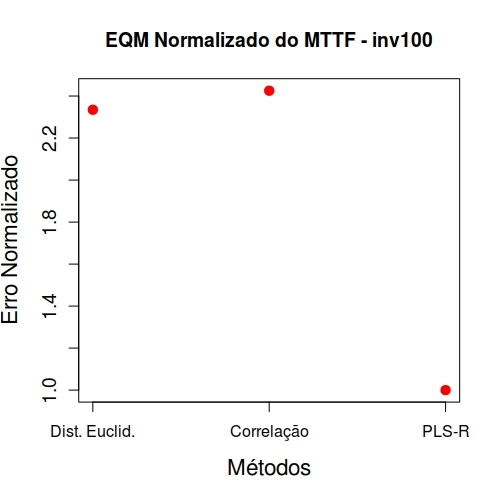
\includegraphics[width=0.5\textwidth]{images/NMSE_MTTF_inv100_random}
	\caption{Erro Quadrático Médio Normalizado do MTTF para a cadeia de inversores.}
	\label{figure:NMSE_MTTF_inv100_random}	
\end{figure}

Entretanto, ao se analisar circuitos de diferentes dimensões, e consequentemente conjuntos de dados de diferença expressiva, algumas das métricas obtidas podem estar em escalas diferentes umas das outras, dificultando a compreensão da precisão dos métodos. Nestes casos, o Erro Normalizado da Raiz do Valor Quadrático Médio facilita a interpretação pois cada conjunto de dados é normalizado pela sua própria média, resultando em um erro percentual. Esse é o caso para a simulação da cadeia de inversores. Sendo substancialmente maior que os demais (de 4 a 10 vezes), seu atraso também é maior e a grandeza, nesse caso, maior. 

O ENRVQM foi extraído para cada circuito e método e estão descritos na tabela \ref{tb:ENRVQM}.

\begin{table}[H]
	\centering
	\caption{Erro Normalizado da Raiz do Valor Quadrático Médio para cada método e circuito em \%.}
	\begin{tabular}{@{}l|l|l|l@{}}
		\toprule
		Circuito & Dist. Eucli. & Cor. & PLS-R \\ \midrule
		inv100 & \ \ \ 13.0\% & 13.1\% & 9.1\% \\
		w\_c499 & \ \ \ 8.1\% & 10.1\% & 8.3\% \\
		w\_c880 &  \ \ \ 7.3\% & 9.6\% & 7.9\% \\
		w\_c1355 & \ \ \ 13.5\% & 18.1\% & 14.7\% \\
		w\_c5315 & \ \ \ 7.9\% & 10.6\% & 8.1\% \\
		\bottomrule
	\end{tabular}
	\label{tb:ENRVQM}
\end{table}

Em seguida foram realizadas simulações de degradação para o BDPE estático mencionada na seção \ref{section:caracterização_iscas} e representado na tabela \ref{tb:BDPE_estatico}. O Erro Normalizado da Raiz do Valor Quadrático Médio para os perfis estáticos se encontram na tabela \ref{tb:ENRVQM_estatico}.
\begin{table}[H]
	\centering
	\caption{ENRVQM para cada método e circuito submetidos à perfis estáticos em \%.}
	\begin{tabular}{@{}l|l|l|l@{}}
		\toprule
		Circuito & Dist. Eucli. & Cor. & PLS-R \\ \midrule
		inv100 & \ \ \ 18.08\% & 18.08\% & 2.07\% \\
		w\_c499 & \ \ \ 22.12\% & 22.12\% & 2.55\% \\
		w\_c880 &  \ \ \ 14.79\% & 14.79\% & 3.00\% \\
		w\_c1355 & \ \ \ 29.76\% & 29.76\% & 4.85\% \\
		w\_c5315 & \ \ \ 15.85\% & 15.85\% & 3.44\% \\
		\bottomrule
	\end{tabular}
	\label{tb:ENRVQM_estatico}
\end{table}

\section{Discussão dos resultados}
Ao se analisar o Erro Relativo (ER) através do diagrama de caixas fica subentendido, inicialmente, que a COR e a DE são métodos mais apropriados. A mediana de ambos os métodos é muito próxima de $0$. Isso é um indicativo de que o ER é muito pequeno em muitos casos. Além disso, a COR parece ser o melhor dos métodos, visto que 75\% dos seus erros relativos estão ``comprimidos'' na região de $ER=0$. 

Entretanto, a quantidade de \textit{outliers} aparenta ser alta. Se a ocorrência de outliers for considerável, isso se refletirá negativamente na precisão dos métodos. Observando a tabela \ref{tb:erro_maximo_ISCAS}, o EMAX dos métodos indica que, quando existe um erro na previsão, ele pode ser de aproximadamente 100\%. Isso significa que o dado estimado $\hat{y_i}$ é até duas vezes maior (ou duas vezes menor) que o ${y_i}$ esperado.

Logo, é preciso averiguar se esses grandes erros de estimativa são usuais para os métodos e dados observados. Se forem, o erro quadrático médio é capaz de enfatizar estes erros. Porém, ao se trabalhar com métricas quadráticas, o resultado não mantém um significado físico plausível. Por este motivo, o resultado é normalizado (EQMN) utilizando o menor erro como referência e apresentado como mostrado na figura \ref{figure:NMSE_MTTF} para facilitar a compreensão.

O EQMN deixa explícito que a Distância Euclideana não é um método tão impreciso quanto indicava o diagrama de caixas do ER. Em adição, a PLS-R mostra-se como um método de precisão comparável à DE. Já a correlação está se mostrando como sendo o pior dos métodos entre os três, sendo até duas vezes mais impreciso que a DE.

Como mencionado na seção \ref{section:metricas_estatisticas}, não há consenso na literatura sobre qual métrica é a mais apropriada para análise de erros de estimativas. Por isso, além do Erro Quadrático Médio, o Erro Normalizado da Raiz do Valor Quadrático Médio também é utilizado, podendo ajudar a compreender um pouco melhor os resultados obtidos. Assim como a figura \ref{figure:NMSE_MTTF}, a tabela \ref{tb:ENRVQM} também indica que a DE e a PLS-R possuem uma precisão semelhante. Entretanto, o ENRVQM médio para DE é de $10\%$ e de $9.6\%$ para a Regressão de Mínimos Quadrados Parciais. Já a Correlação apresenta um ENRVQM médio de $12.3\%$ e consolida-se como o pior método para estimativa.

Esses resultados mostram que uma estratégia proativa para extensão do tempo de vida de um sistema que utilize a Distância Euclideana ou PLS-R como método de estimativa pode ter uma precisão de aproximadamente 90\%. Esta performance pode ser melhorada ainda mais à medida que o BDPE for atualizado com dados de campo. A metodologia, ao propor uma modularização do sistema (conforme descrito na seção \ref{section_visao_geral}) permite que os próprios modelos sejam atualizados ou substituídos, potencialmente melhorando ainda mais a precisão.

Ao repetirmos esta análise para um BDPE estático, a tabela \ref{tb:ENRVQM_estatico} evidencia que o Erro Normalizado da Raiz do Valor Quadrático Médio para a DE e COR piora bastante. Não é surpreendente um banco que possui poucas entradas, e um espaço amostral tão baixo, afetar estes dois métodos. Ao calcular-se a DE, por exemplo, a distância obtida será igual em todos os casos. Assim, qualquer um dos perfis pode ser enquadrado na condição de ``mais próximo'', o que não é satisfatório.

Adicionalmente, o ENRVQM para a PLS-R mostra-se muito melhor. Observando-se as três primeiras linhas da tabela \ref{tb:BDPE_estatico}, é  possível perceber que a tensão de alimentação mantém-se a mesma, enquanto a temperatura pode apresentar apenas os valores de 40, 70 e 100. O mesmo pode ser observado para o restante dos dados. Separando estas informações em grupos que possuem a mesma tensão de alimentação, a dependência do atraso de saída pela temperatura para diferentes $V_{DD}$ é dada pela figura \ref{figure:Temp_atraso_VDDcte}.
\begin{figure}[H]
	\center
	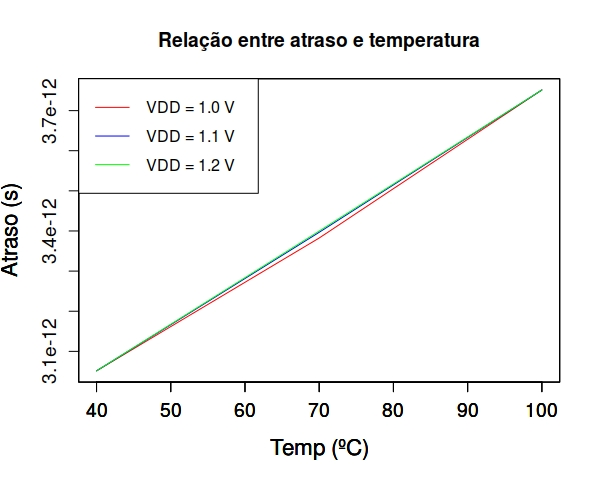
\includegraphics[width=0.8\textwidth]{images/Temp_atraso_VDDcte}
	\caption{Relação entre o atraso e a temperatura para diferentes $V_{DD}$.}
	\label{figure:Temp_atraso_VDDcte}	
\end{figure}

A decomposição dos dados exposta na figura \ref{figure:Temp_atraso_VDDcte} possui uma serventia didática apenas, pois facilita visualizar a relação linear existente entre temperatura e atraso (e consequentemente MTTF). Similarmente, o mesmo pode ser feito entre a tensão de alimentação e o atraso. Se há uma relação linear tão evidente entre estas variáveis explicativas (Temperatura e Tensão) e a variável observada (Atraso ou MTTF), o modelo de PLS-R extraído será consequentemente bem mais preciso.

Este é o motivo pelo qual o ENRVQM para um BDPE estático é mais preciso do que para um BDPE dinâmico. É necessário ressaltar que o um banco de dados de perfis estático considera uma estatística (possivelmente média) para as condições ambientais, sendo bem menos fiel ao verdadeiro perfil de operação de um sistema.

\section{Críticas ao método}
O método apresentado propõe a utilização de diferentes unidades para realizar a tarefa de predição, conforme mostrado na figura \ref{figure:sistema_proposta_metodologia}. Apesar de essa abordagem se mostrar como uma vantagem, permitindo que suas diversas unidades sejam customizadas, melhoradas ou mesmo completamente substituídas, alguns de seus aspectos não estão bem definidos.

Não está definido, por exemplo, se existe uma dimensão recomendada para o BDPE dinâmico. Na análise realizada foram utilizados aproximadamente 250 perfis. Não há entretanto uma motivação específica. Usualmente 30 ou mais amostras são mais do que suficientes para que a distribuição amostral da média de uma população seja considerada uma distribuição \textit{gaussiana} \cite{Montgomery2011}. Entretanto, uma quantidade inferior não garante que a distribuição da estatística será ``não-normal''.

No contexto desse trabalho, essa estatística pode ser o acréscimo médio no atraso $t_d$ ou o MTTF médio. Independente de qual estatística seja escolhida pode-se realizar a análise de um BDPE dinâmico reduzido, com uma quantidade de amostras inferiores e averiguar como os métodos se comportam. Após repetir esta análise com apenas 28 perfis, evitando a garantia de normalidade da média, o ENRVQM obtido para os circuitos e métodos é apresentado na tabela \ref{tb:ENRVQM_reduzido}.

\begin{table}[H]
	\centering
	\caption{ENRVQM para cada método e circuito submetidos à 28 perfis dinâmicos.}
	\begin{tabular}{@{}l|l|l|l@{}}
		\toprule
		Circuito & Dist. Eucli. & Cor. & PLS-R \\ \midrule
		inv100 & \ \ \ 14.89\% & 15.89\% & 7.61\% \\
		w\_c499 & \ \ \ 21.99\% & 26.13\% & 9.21\% \\
		w\_c880 &  \ \ \ 21.25\% & 22.55\% & 8.87\% \\
		w\_c1355 & \ \ \ 14.23\% & 16.49\% & 14.86\% \\
		w\_c5315 & \ \ \ 17.99\% & 19.41\% & 8.95\% \\
		\bottomrule
	\end{tabular}
	\label{tb:ENRVQM_reduzido}
\end{table}

O ENRVQM médio para a DE é de 18.07\% e para a PLS-R é de 9.9\%. Para a COR é obtido um ENRVQM médio de 20.09\%. Apesar de a PLS-R se manter como o melhor método, a diferença para a DE é considerável desta vez. Então a crítica ao método se mantém e levanta alguns questionamentos:
\begin{enumerate}
	\item Qual é a dimensão do BDPE necessária para que se tenha uma boa predição?
	\item Aumentar o BDPE ainda mais garantirá que a DE se torne um método melhor que a PLS-R eventualmente?
	\item Qual é a relação existente entre o aumento do BDPE e a redução dos erros de predição para cada método?
\end{enumerate}